\documentclass[esd, manuscript]{copernicus} % uncomment to see what the 2 column final paper will look like.

\begin{document}

\section{The emulator}

We treat the output of the simulator $y$ as an uncertain function $f()$ of the simulator inputs $x$, so that $y = f(x)$. We wish to produce a predictive distribution for $y$ at any model input, conditional on the points already run, or the design $(Y, X)$. Throughout the study, we use a kriging function, similar to a Gaussian process regression emulator, as coded in the R package DiceKriging \citep{roustant2012dicekriging} for prediction of climate simulator output at untried inputs.
The kriging model or Gaussian Process regression is specified hierarchically with a separate mean and covariance function. For prediction purposes, \emph{a priori} assume that the trend is a simple linear function of the inputs, and adjust with a Gaussian process. 

%\begin{equation}
$$
f(x) = h(x)^T \beta + Z(x)
$$
%\end{equation}

Where $h(x)^T \beta$ is the mean function, and the residual process $Z$ is a zero mean stationary Gaussian process. The covariance kernel $c$ of $Z$ 

$$
Cov(Z, Z') = \sigma^2 c(x,x')
$$
can be specified in a number of different ways: we use the default diceKriging option of a Matern $v=5/2$ function so that

$$
c(x,x') = (1 + \frac{\sqrt{5} | x - x'|}{\theta} + \frac{5 | x - x'|^2}{3 \theta^2})exp(- \frac{\sqrt{5} |x-x'|}{\theta})
$$

where $\theta$ describes the \emph{characteristic length scales} - a measure of how quickly information about the function is lost moving away from a design point, in any dimension. This and other hyperparameters are estimated via maximum likelihood estimation from the design $(Y, X)$, meaning that the approach is not fully Bayesian (such an approach would find posterior distributions for the hyperparameters rather than point estimates). We use Universal Kriging, with no `nugget' term, meaning that the uncertainty on model outputs shrinks to zero at the design points. 

Full details of the Universal kriging process used can be found in \citep{roustant2012dicekriging}, section 2.1, details of the kernel can be found in section 2.3, and examples of the trend and hyperparameter estimation  in section 3 the same publication. 

\subsection{Testing the emulator}
To ensure that the emulator is adequate for prediction, we need to ensure that it predicts well across the parameter space of the design $X$. We use leave-one-out cross validation (LOOCV), where each ensemble member is removed in turn, and the output $y$ predicted with an emulator constructed from the remaining design points. This type of validation quickly shows up any design points where the emulator fails badly, either in the mean prediction, or in the assessed uncertainty. This, and other standard model selection and validation metrics can be found in e.g. chapter 7 of \citep{hastie2009elements}.

Cross validation of the emulator for forest fraction shows up no significant problems in prediction of any of the global or regional forest fraction data, across the entire design, as can be seen in figure \ref{fig:frac_loo}.


\bibliographystyle{copernicus}
\bibliography{famous.bib}

\begin{figure}[t]
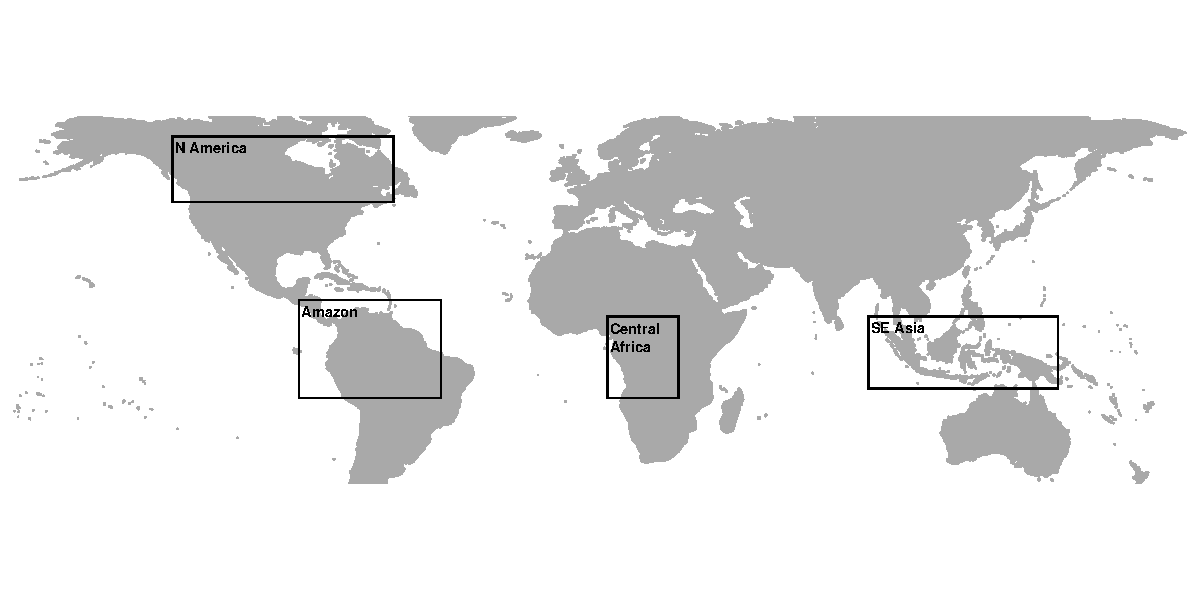
\includegraphics[width=12cm]{graphics/map_forests.pdf}
\caption{A map of the forest regions used in the study. Regions are: Amazon 15\textdegree S - 15\textdegree N, 270\textdegree E - 315\textdegree E; Central Africa; 15\textdegree S - 10\textdegree N, 7.5\textdegree E - 30\textdegree E; SE Asia 12\textdegree S - 10\textdegree N, 90\textdegree E - 150\textdegree E; North America 45\textdegree N - 65\textdegree N, 230\textdegree E - 300\textdegree E.}
\label{fig:map_forests}
\end{figure}

\begin{figure}[t]
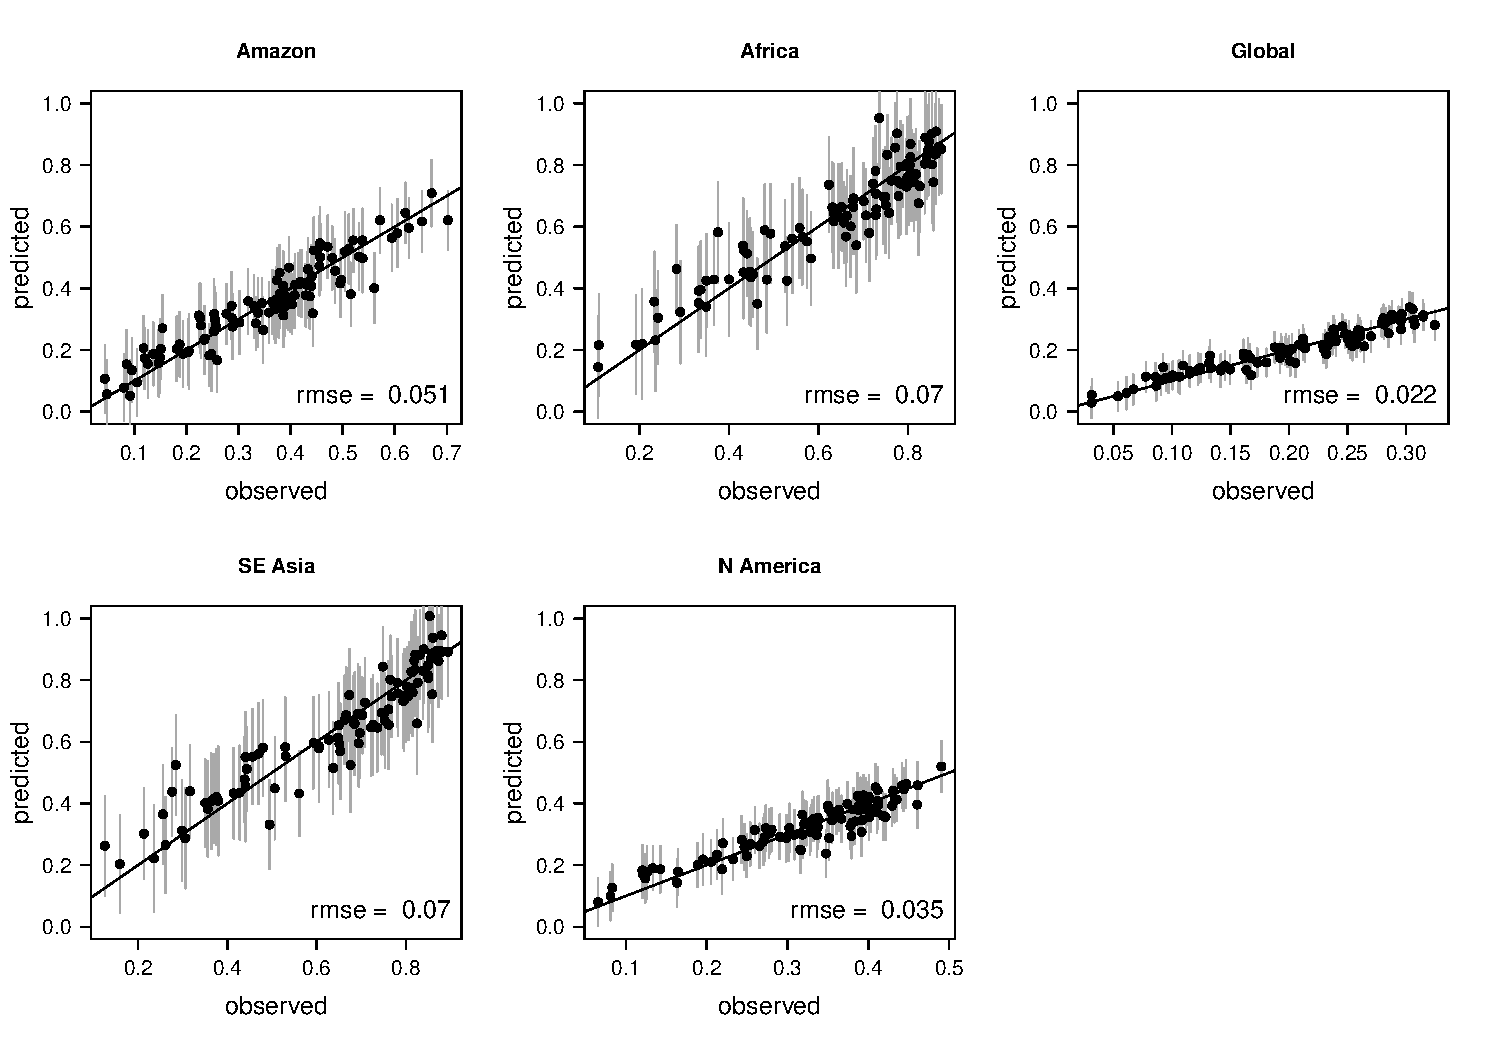
\includegraphics[width=12cm]{graphics/frac_loo.pdf}
\caption{Leave-one-out cross validation performance of the emulator, when reproducing each forest fraction. Black points represent the emulator central estimate of a held-out point, with grey lines representing $\pm$ 2 standard deviations.}
\label{fig:frac_loo}
\end{figure}



\end{document}